\chapter{Code Smells}

\section{代码异味}

代码异味指的是代码中的某些特征,这些特征可能表明设计的质量存在问题。它不是明确的错误,而是代码中可能存在问题的迹象。

代码异味是基于启发式的,这意味着它们不是固定不变的规则。启发式原则提供了一个初步的方法或指引,但不保证总是正确。
因此,当我们在代码中发现异味时,不意味着一定存在问题,但确实表明我们需要更仔细地查看这部分代码,以确定是否真的存在设计问题。

这个概念源自Martin Fowler的书《Refactoring: Improving the design of existing code》。这本书是关于重构的,重构是一个软件工程的实践,目的是在不改变外部行为的前提下,改进代码的内部结构。
在这本书中,代码异味章节是由Martin Fowler与Kent Beck共同撰写的。Kent Beck是敏捷开发和测试驱动开发的先驱,与Martin Fowler一同在软件工程领域有着重要的影响。

\section{常见的代码异味}

\subsection{重复代码 (Duplicate Code)}这是最常见的代码异味。当在代码库中有重复的代码片段时,任何对这些代码的更改都需要在多个位置进行,增加了维护的复杂性。
\paragraph{修复方法}重构技术,如“提取方法”或“提取类”可以帮助消除重复代码。

\subsection{长方法 (Long Method)}当一个方法太长时,它通常做了太多的事情,违反了“单一职责原则”。
\paragraph{修复方法}可以通过“提取方法”重构来分解长方法,将其拆分成多个更小、更具描述性的方法。

\subsection{大类 (Large Class)}类似于长方法,一个类如果太大,可能承担了太多的职责。
\paragraph{修复方法}可以通过“提取类”重构来将大类分解为几个小类,每个类都有其明确的职责。

\subsection{长参数列表 (Long Parameter List)}方法有太多的参数,增加了理解和使用该方法的复杂性。
\paragraph{修复方法}使用参数对象或其他重构技术减少参数数量。

\subsection{投机性泛化 (Speculative Generality)}代码中包含的某些构造、功能或参数,是为了泛化类、方法或设计。并不是因为当前的需求,而是基于未来可能的需求。
\paragraph{修复方法}删除未使用的代码或将其简化。

\subsection{数据类 (Data Class)}这些类只有字段(属性)但缺乏行为。这可能意味着代码的其他部分是在不恰当的地方处理与这些数据相关的逻辑。
\paragraph{修复方法}向数据类添加方法,或将相关逻辑移到适当的地方。

\subsection{注释作为除臭剂 (Comments as deodorant)}过度依赖注释来解释复杂或不清晰的代码。
\paragraph{修复方法}重构代码使其更具可读性,而不是仅依赖注释。

\subsection{临时字段 (Temporary Field)}这些字段只在某些特定条件下使用,可能会导致代码难以理解和出错。考虑使用更清晰的数据结构或对象,或重新考虑该逻辑。
\paragraph{修复方法}考虑使用更清晰的数据结构或对象,或重新考虑该逻辑。

\section{常见现象及对应的代码异味}
\subsection{Large Class}
“大类”是指在设计中,类的大小超过了它应有的范围,从而可能导致一些设计上的问题。但是,“大”是一个相对的概念,取决于上下文和项目的规模。

使用LOC(Lines of Code,代码行数)或其他绝对度量标准来定义类的大小可能不是一个好方法。因为对于一个10,000行代码的系统,一个100行的类可能不算大;但对于一个只有300行代码的系统,100行的类就显得很大了。

\subsubsection{大类可能带来的问题}

\paragraph{更高的变更风险(CR)}当类变得越大,它占据的代码总量也会增加。这意味着,在多种变更场景下,这个类都可能需要进行修改,从而增加了变更风险(Change Risk,CR)。这进一步降低了代码的可修改性(alterability)。

\paragraph{违反单一职责原则(SRP)}单一职责原则建议一个类只应有一个引起它变化的原因。当类过大时,它可能涉及多个功能或职责,从而违反了SRP。

\paragraph{更高的耦合度}大类可能与多个其他类交互,从而增加了耦合度。高耦合度意味着修改一个类可能会影响到其他类,这使得代码维护变得更困难。

\paragraph{可能的低内聚度}内聚度指的是一个类的各个部分(如方法或属性)如何紧密地关联在一起。当类很大时,它的各个部分可能并不都是为了同一目标而工作,导致低内聚度。这也可能使得类难以理解和维护。

\subsubsection{相关的代码异味}
\paragraph{长方法}方法越长,类就必须越大,从而导致大类。
\paragraph{长参数列表}参数越多,方法越长,从而导致长方法。

采用启发式方法的一个困难是不知道何时采用;另一个困难是不知道具体该怎么做。

\subsection{未封装的集合类}

``Unencapsulated Collection" 是一种设计问题,指的是在代码中直接使用通用集合(如List、Set、Map等)来表示特定于上下文的集合数据,而没有提供适当的封装。这种做法可能会导致多种问题,包括不一致性、潜在的错误、代码重复、低内聚,以及暴露了实现细节。

使用通用集合类,如java.util.List,可能允许对集合进行意外或非法的修改,这些修改违反了context schema规则或期望(例如,一旦创建,纸牌的一副牌应该永远不会改变)。因此,这可能是错误的来源,因为集合可以以与上下文模式不一致的方式被更改。

\paragraph{代码重复和内聚性降低}当集合未被适当封装时,任何需要处理集合的客户端代码都必须提供执行必要处理的代码。如果多个客户端需要执行相同的操作,这将导致代码重复。由于客户端代码必须处理与集合相关的各种任务,这可能会导致低内聚,因为代码必须管理与其主要责任不一致的多个任务。

直接使用通用集合暴露了实现细节。这违反了封装的原则,即实现细节应该对使用类的客户端隐藏。这种暴露使得将来更改集合的实现(例如,从List更改为Set)会更加困难,因为这需要更改客户端代码。

针对这些问题,最佳的解决方案是封装集合。这意味着:

\textbf{创建自定义类:}
为特定的集合创建自定义类,封装内部的通用集合。这个类应该提供特定于上下文的方法来管理集合,而不是暴露集合本身或其全套操作。

\textbf{控制对集合的访问:}
通过只提供必要的方法来操作集合数据,可以预防不符合上下文规则的修改。例如,如果集合不应被修改,则不提供添加或删除元素的方法。

\textbf{降低客户端的复杂性:}
封装集合后,客户端代码不再直接与集合交互,而是通过明确定义的接口,从而简化客户端的逻辑并提高内聚度。

\textbf{隐藏实现细节}:
封装也有助于隐藏实现细节,使得未来对集合的实现做出更改时,客户端代码不需要做出修改,提高了代码的可维护性和灵活性。

\subsubsection{封装集合}

创建一个类来代表特定上下文模式的集合:
这一步是面向对象设计的基础,即识别并封装变化。在这种情况下,我们正在处理的不仅仅是一个通用的集合,而是在特定上下文(如书籍、订单、学生等)中具有特定意义和行为的集合。创建一个代表此集合的类可以增加代码的可读性、可维护性,并减少错误,因为这个类将确保所有操作都符合预期的业务规则。

使未封装的集合成为新类的一个字段:
这一步涉及到将通用集合(如List<Book>)封装在新类内部。这样做的目的是限制对集合的直接访问和修改,只允许通过定义好的接口(即新类的方法)来进行操作。这种封装保护了数据的完整性,并确保了数据的使用方式符合业务逻辑。

将处理集合的代码(相关部分)移动到新类的方法中:
这是重构过程中的关键一步,涉及到代码的重新组织。之前散布在客户端代码中处理集合的逻辑现在被整合并移动到新类的方法中。这不仅减少了代码重复,还提高了代码的内聚性,因为相关的行为现在被组织在一起。

调整客户端代码以使用新类:
客户端代码需要被重构,以便使用新类的方法而不是直接操作集合。这一步可能需要一些努力,特别是当原始的未封装集合在系统的多个地方被使用时。然而,长远来看,这将大大提高代码的可维护性和可扩展性,同时降低错误率。

\subsubsection{封装集合后对可维护性的影响}

内聚提升了,导致可理解性的提升;封装意味着不能以意料之外的方式更改集合,也意味着可理解性的提升;更短的方法以及更有意义的方法名同样提升了可理解性。

N增加了,也就是CR减少了,意味着可变性的增加。

测试可独立于客户代码进行,可测试性也增加了。

\section{总结}
理解代码异味和重构的重要性对于任何希望编写高质量、可维护代码的开发者来说都是至关重要的。虽然代码异味是通过启发式识别的,可能需要开发者的判断,但重构通常是提高代码质量的关键步骤。

一个常见的设计决定(又称 "设计气味")是围绕一个项目集合,然后以不同的方式处理该集合---一个未封装的集合。

通过重构将集合封装起来,创建一个以集合为字段的类,并使用类中的方法进行所需的不同处理,从而消除气味。

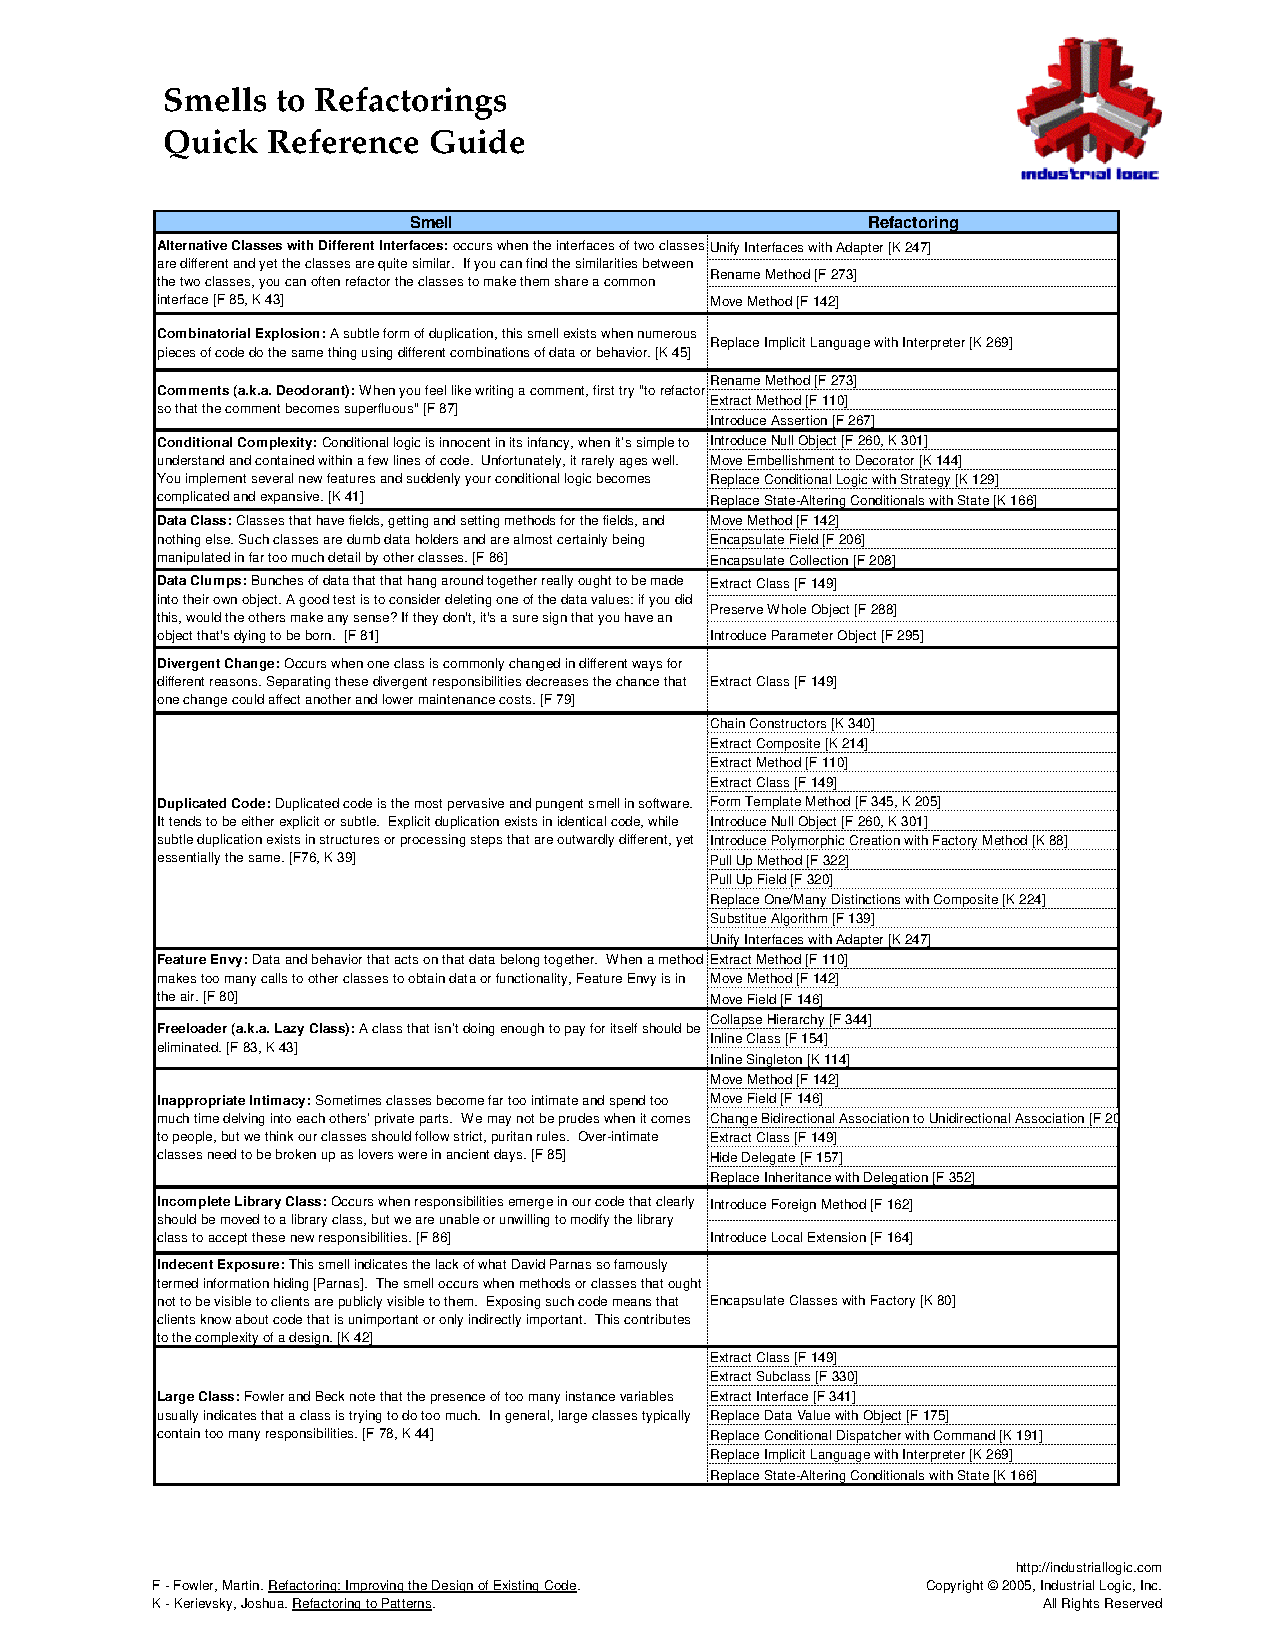
\includepdf[pages={1,2}]{res/smellstorefactorings.pdf}




























